\documentclass[11pt,a4paper]{article}

% ---------------- PACKAGES ----------------
\usepackage[utf8]{inputenc}
\usepackage[T1]{fontenc}
\usepackage[french]{babel}
\usepackage{amsmath, amssymb}
\usepackage{siunitx}
\usepackage{geometry}
\usepackage{multicol}
\usepackage{tcolorbox}
\usepackage{tikz}
\usepackage{xcolor}
\usepackage{fancyhdr}

\geometry{margin=2cm}
\pagestyle{fancy}
\fancyhf{}
\lhead{\textbf{Puissance et Énergie}}
\rhead{\thepage}

% ---------------- COLORS ----------------
\definecolor{energyblue}{RGB}{30,80,160}
\definecolor{powerred}{RGB}{180,50,50}
\definecolor{warningred}{RGB}{200,30,30}
\definecolor{graybg}{RGB}{245,245,245}

% ---------------- TCOLORBOX ----------------
\tcbset{
  sharp corners,
  colback=white,
  colframe=black!60,
  boxrule=0.8pt,
  left=6pt, right=6pt, top=4pt, bottom=4pt
}

\newcommand{\theorybox}[2]{
\begin{tcolorbox}[title=\textbf{#1}]
#2
\end{tcolorbox}
}

% ---------------- EXERCISE GRIDS ----------------
\newcommand{\fullgrid}{
\vfill
\begin{center}
\begin{tikzpicture}[scale=0.9]
\draw[step=0.5cm,gray!30,very thin] (0,0) grid (18,22);
\end{tikzpicture}
\end{center}
\vfill
}

\newcommand{\threequartergrid}{
\vfill
\begin{center}
\begin{tikzpicture}[scale=0.9]
\draw[step=0.5cm,gray!30,very thin] (0,0) grid (18,18);
\end{tikzpicture}
\end{center}
\vfill
}

\begin{document}

\section*{Pompage-turbinage et économie de l’énergie}

Cet exercice étudie le fonctionnement simplifié du système hydroélectrique
de pompage-turbinage entre le lac de Hongrin et le lac Léman.

Le système fonctionne de la manière suivante :
\begin{figure}
    \centering
    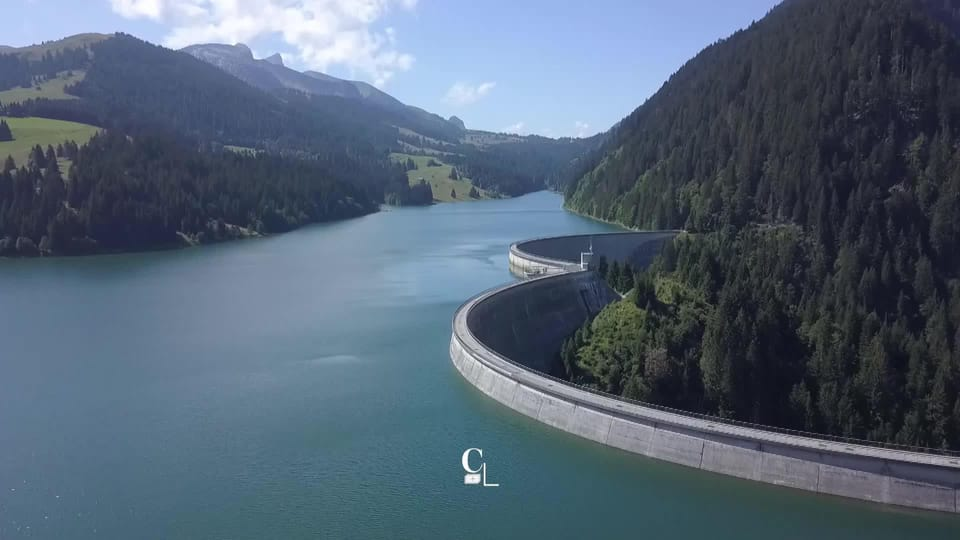
\includegraphics[width=0.75\linewidth]{barage.jpeg}
    \caption{Le Barrage de l'Hongrin, source : RTS}
\end{figure}
\begin{itemize}
\item La nuit, l’électricité est bon marché et des pompes sont utilisées pour remonter l’eau
du lac Léman vers le réservoir du lac de Hongrin.
\item Pendant la journée, l’eau stockée redescend à travers des turbines
pour produire de l’électricité lorsque le prix de l’électricité est plus élevé.
\end{itemize}

Cela permet de \textbf{stocker de l’énergie et de la revendre plus tard}.

Prix de l’électricité :

\begin{itemize}
\item Nuit (00h00 -- 07h00) : $15\,\si{ct/kWh}$
\item Jour (07h00 -- 24h00) : $35\,\si{ct/kWh}$
\end{itemize}

Caractéristiques du système :

\begin{itemize}

\item Surface du lac de Hongrin : $1.6\,\si{km^2}$
\item Profondeur moyenne du lac : $30\,\si{m}$
\item Différence de hauteur avec le lac Léman : $900\,\si{m}$

\item Puissance maximale de la turbine : $500\,\si{MW}$
\item Puissance maximale des pompes : $400\,\si{MW}$

\item Rendement turbine + générateur : $90\%$
\item Rendement des pompes : $80\%$

\item Apport annuel d’eau dans le réservoir :
$150\,\text{millions } \si{m^3 / an}$

\item Consommation électrique moyenne d’un foyer :
$4500\,\si{kWh/an}$

\item Consommation d’une voiture électrique :
$150\,\si{Wh/km}$

\end{itemize}

Tous les calculs doivent être effectués en \textbf{unités du SI}.

\newpage

\subsection*{Partie A - Volume du réservoir}

Nous commençons par estimer le volume d’eau contenu dans le lac.

\begin{itemize}

\item Convertir la surface du lac de $\si{km^2}$ en $\si{m^2}$.

\item Identifier la profondeur moyenne du lac.

\item Calculer le volume total d’eau stocké dans le réservoir.

\item Exprimer le résultat en $\si{m^3}$.

\end{itemize}

\threequartergrid

\newpage
\subsection*{Partie B - Énergie potentielle stockée dans le lac}

L’eau du réservoir se trouve environ $900\,\si{m}$ au-dessus du lac Léman.

Cela signifie que l’eau possède une énergie potentielle gravitationnelle.

\begin{itemize}

\item Déterminer la masse totale d’eau contenue dans le réservoir
(en utilisant la densité de l’eau).

\item Identifier la différence de hauteur entre les deux lacs.

\item Calculer l’énergie gravitationnelle totale stockée dans le réservoir.

\item Exprimer le résultat en joules.

\item Convertir cette énergie en $\si{kWh}$.

\end{itemize}

\threequartergrid

\newpage
\subsection*{Partie C - Puissance électrique maximale}

Lorsque l’eau redescend, les turbines produisent de l’électricité.

\begin{itemize}

\item Identifier la puissance mécanique maximale disponible sur la turbine.

\item Tenir compte du rendement turbine + générateur.

\item Calculer la puissance électrique maximale fournie au réseau.

\item Exprimer le résultat en $\si{MW}$.

\end{itemize}

\threequartergrid

\newpage
\subsection*{Partie D - Production d’énergie quotidienne}

Supposons que les turbines fonctionnent à puissance maximale pendant la journée.

\begin{itemize}

\item Déterminer la durée de la période de marché de l’électricité en journée.

\item Calculer l’énergie électrique maximale pouvant être produite
pendant une journée.

\item Exprimer le résultat en $\si{kWh}$.

\end{itemize}

\threequartergrid

\newpage
\subsection*{Partie E - Énergie de pompage pendant la nuit}

Pendant la nuit, de l’électricité est utilisée pour remonter l’eau vers le réservoir.

\begin{itemize}

\item Déterminer la durée de la période nocturne.

\item Identifier la puissance électrique maximale des pompes.

\item Calculer l’énergie électrique utilisée par les pompes chaque nuit.

\item Tenir compte du rendement des pompes pour déterminer
l’énergie gravitationnelle réellement stockée dans l’eau.

\end{itemize}

\threequartergrid

\newpage
\subsection*{Partie F - Profit économique quotidien}

Le but du pompage-turbinage est d’acheter de l’électricité lorsqu’elle est bon marché
et de la revendre lorsqu’elle est plus chère.

\begin{itemize}

\item Calculer le coût de l’électricité utilisée pour le pompage pendant la nuit.

\item Calculer la valeur de l’électricité vendue pendant la journée.

\item Tenir compte des rendements.

\item Calculer le profit net pour un cycle complet d’une journée.

\item Exprimer le résultat en francs suisses par jour.

\end{itemize}

\threequartergrid

\newpage
\subsection*{Partie G - Combien de foyers peuvent être alimentés ?}

Nous estimons maintenant combien de foyers peuvent être alimentés.

\begin{itemize}

\item Utiliser l’apport annuel d’eau dans le réservoir.

\item Calculer l’énergie gravitationnelle totale disponible chaque année.

\item Tenir compte du rendement des turbines pour déterminer
l’énergie électrique produite.

\item Convertir le résultat en $\si{kWh/an}$.

\item Comparer cette valeur avec la consommation annuelle
d’un foyer.

\item Déterminer combien de foyers pourraient être alimentés.

\end{itemize}

\threequartergrid

\newpage
\subsection*{Partie H - Équivalent en voitures électriques}

Enfin, nous comparons cette énergie avec la mobilité électrique.

\begin{itemize}

\item Utiliser l’énergie électrique totale stockée dans le lac.

\item Convertir l’énergie en watt-heures.

\item Utiliser la consommation moyenne d’une voiture électrique.

\item Calculer la distance totale pouvant être parcourue avec
cette énergie.

\item Exprimer le résultat en kilomètres.

\end{itemize}

\threequartergrid

\end{document}